
    \begin{picture} (180.000000,180.000000)(0,0)
    \put(0.0, 0.0){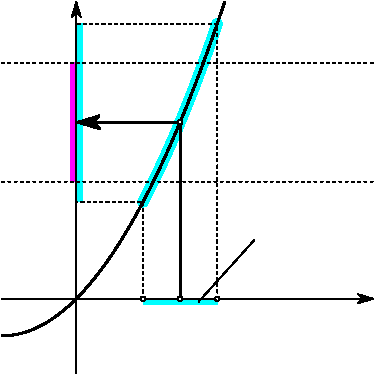
\includegraphics{03epsAndDeltaTooBig.pdf}}
        \put( -2.00,  92.85){\sffamily\itshape \makebox[0pt][r]{$L-\varepsilon$}}
    \put( -2.00, 149.81){\sffamily\itshape \makebox[0pt][r]{$L+\varepsilon$}}
    \put( 31.60, 121.33){\sffamily\itshape \makebox[0pt][r]{$L$}}
    \put(108.24, 168.50){\sffamily\itshape $y=f(x)$}
    \put(107.24,  39.60){\sffamily\itshape $a+\delta$}
    \put( 44.64,  39.60){\sffamily\itshape $a-\delta$}
    \put( 84.44,  24.60){\sffamily\itshape $a$}
    \put(125.04,  64.72){\sffamily\itshape \begin{minipage}{240pt}
        For some $x$ in this interval $f(x)$ is not between
        $L-\varepsilon$ and $L+\varepsilon$. Therefore the $\delta$ in this
        picture is too big for the given $\varepsilon$.  You need a smaller
        $\delta$.
        \end{minipage}}
\end{picture}
